\section{Thrust 3. Voice-Driven Features for an IDE to support VIPLs}
\label{sec:thrust3}

\begin{figure}[t]
\centering
\begin{minipage}{.48\textwidth}
%\begin{figure}[t]
\centering
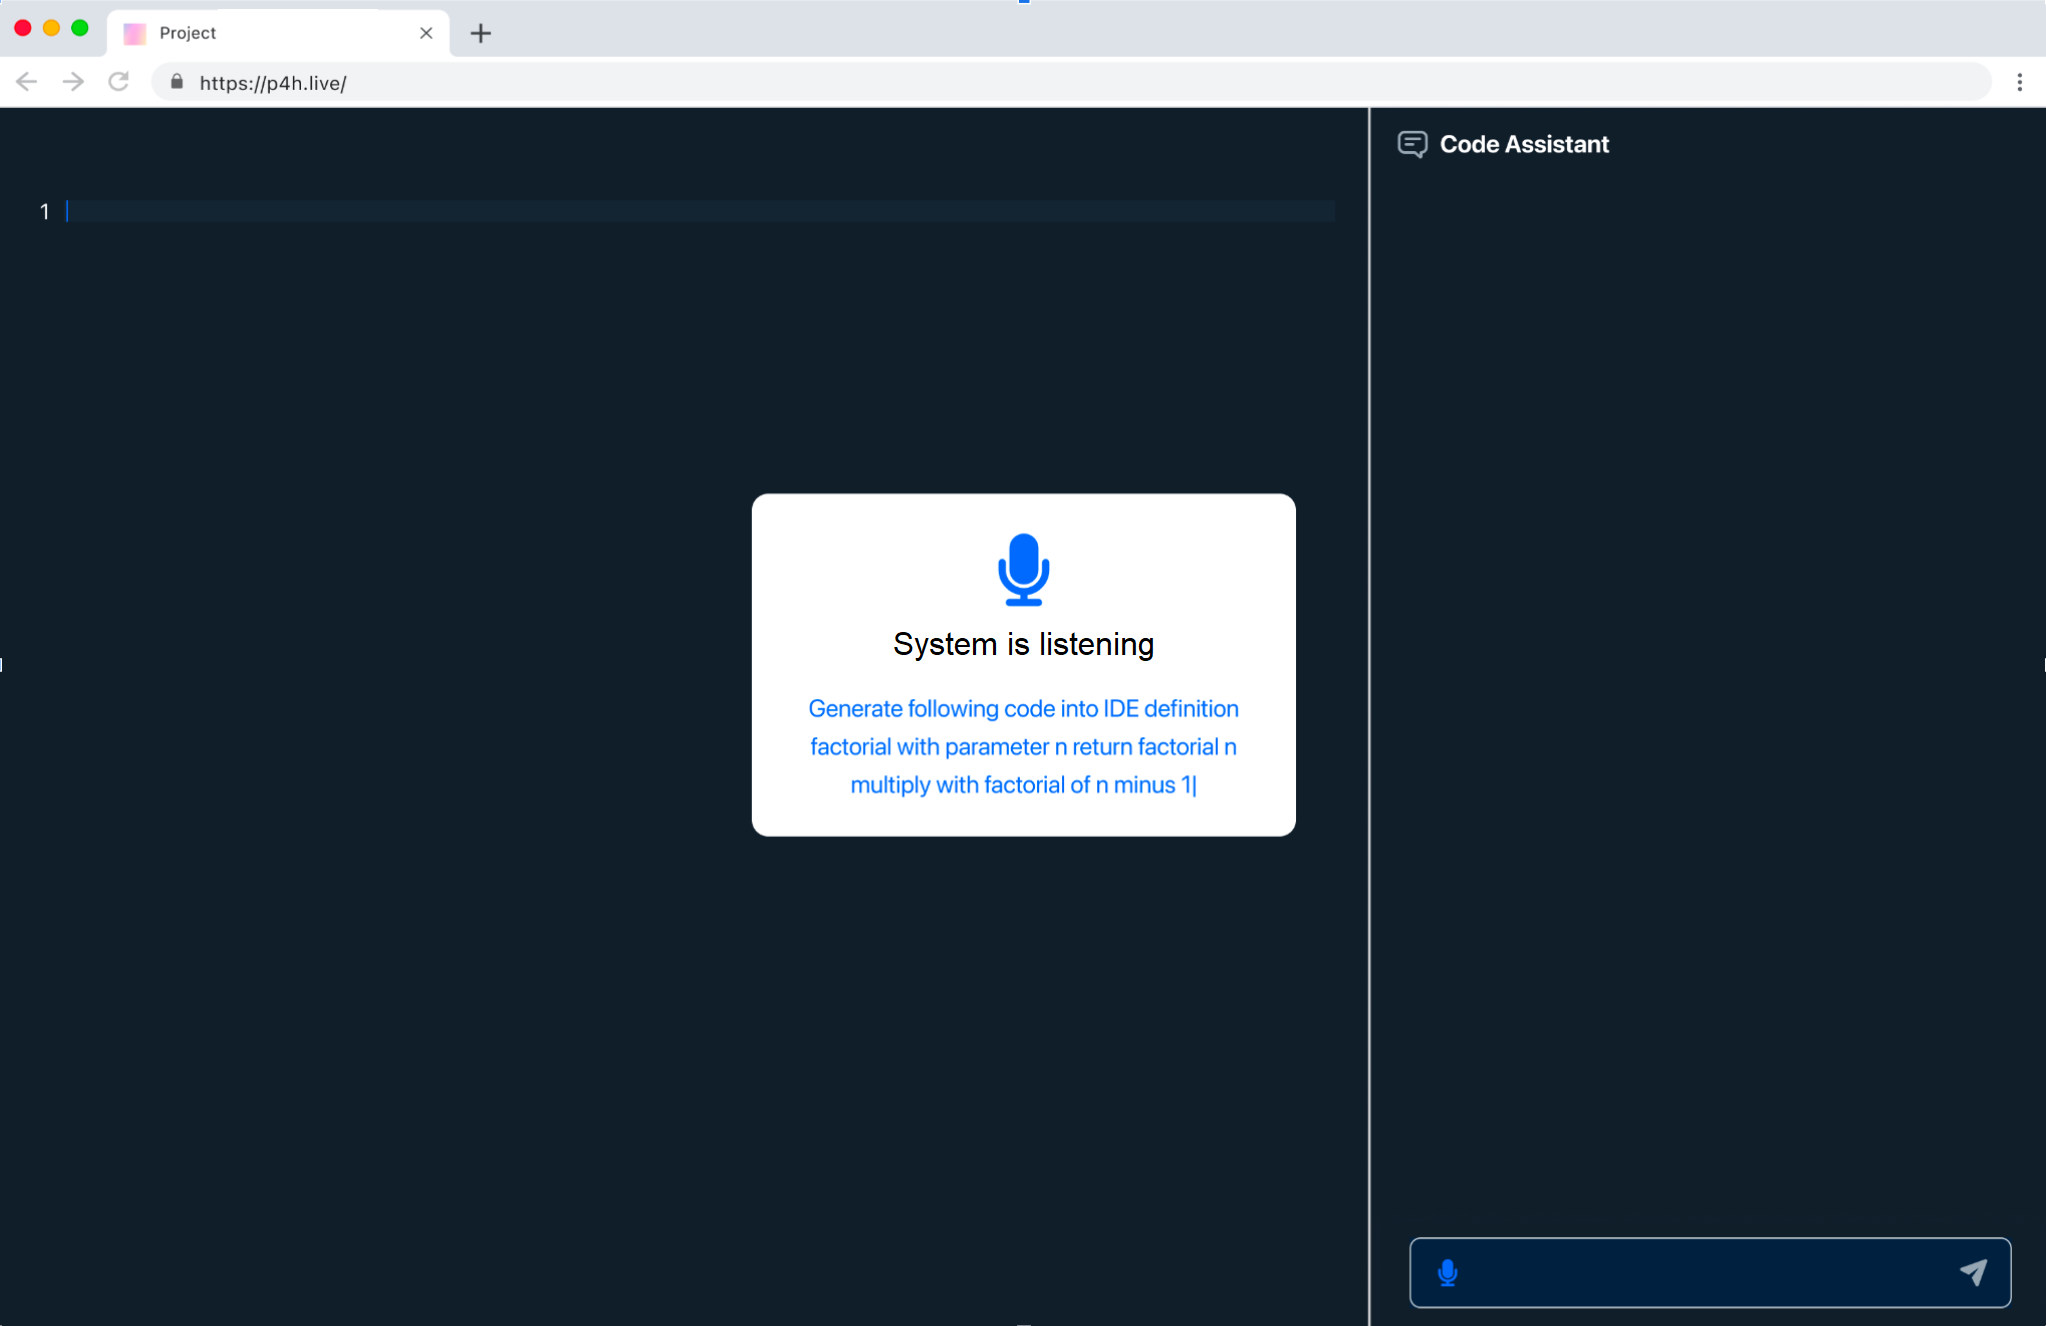
\includegraphics[width=.98\textwidth]{p4h-1}
%\caption{caption 1}
%\label{fig:left}
%\end{figure}
\end{minipage}
\begin{minipage}{.48\textwidth}
%\begin{figure}[t]
\centering
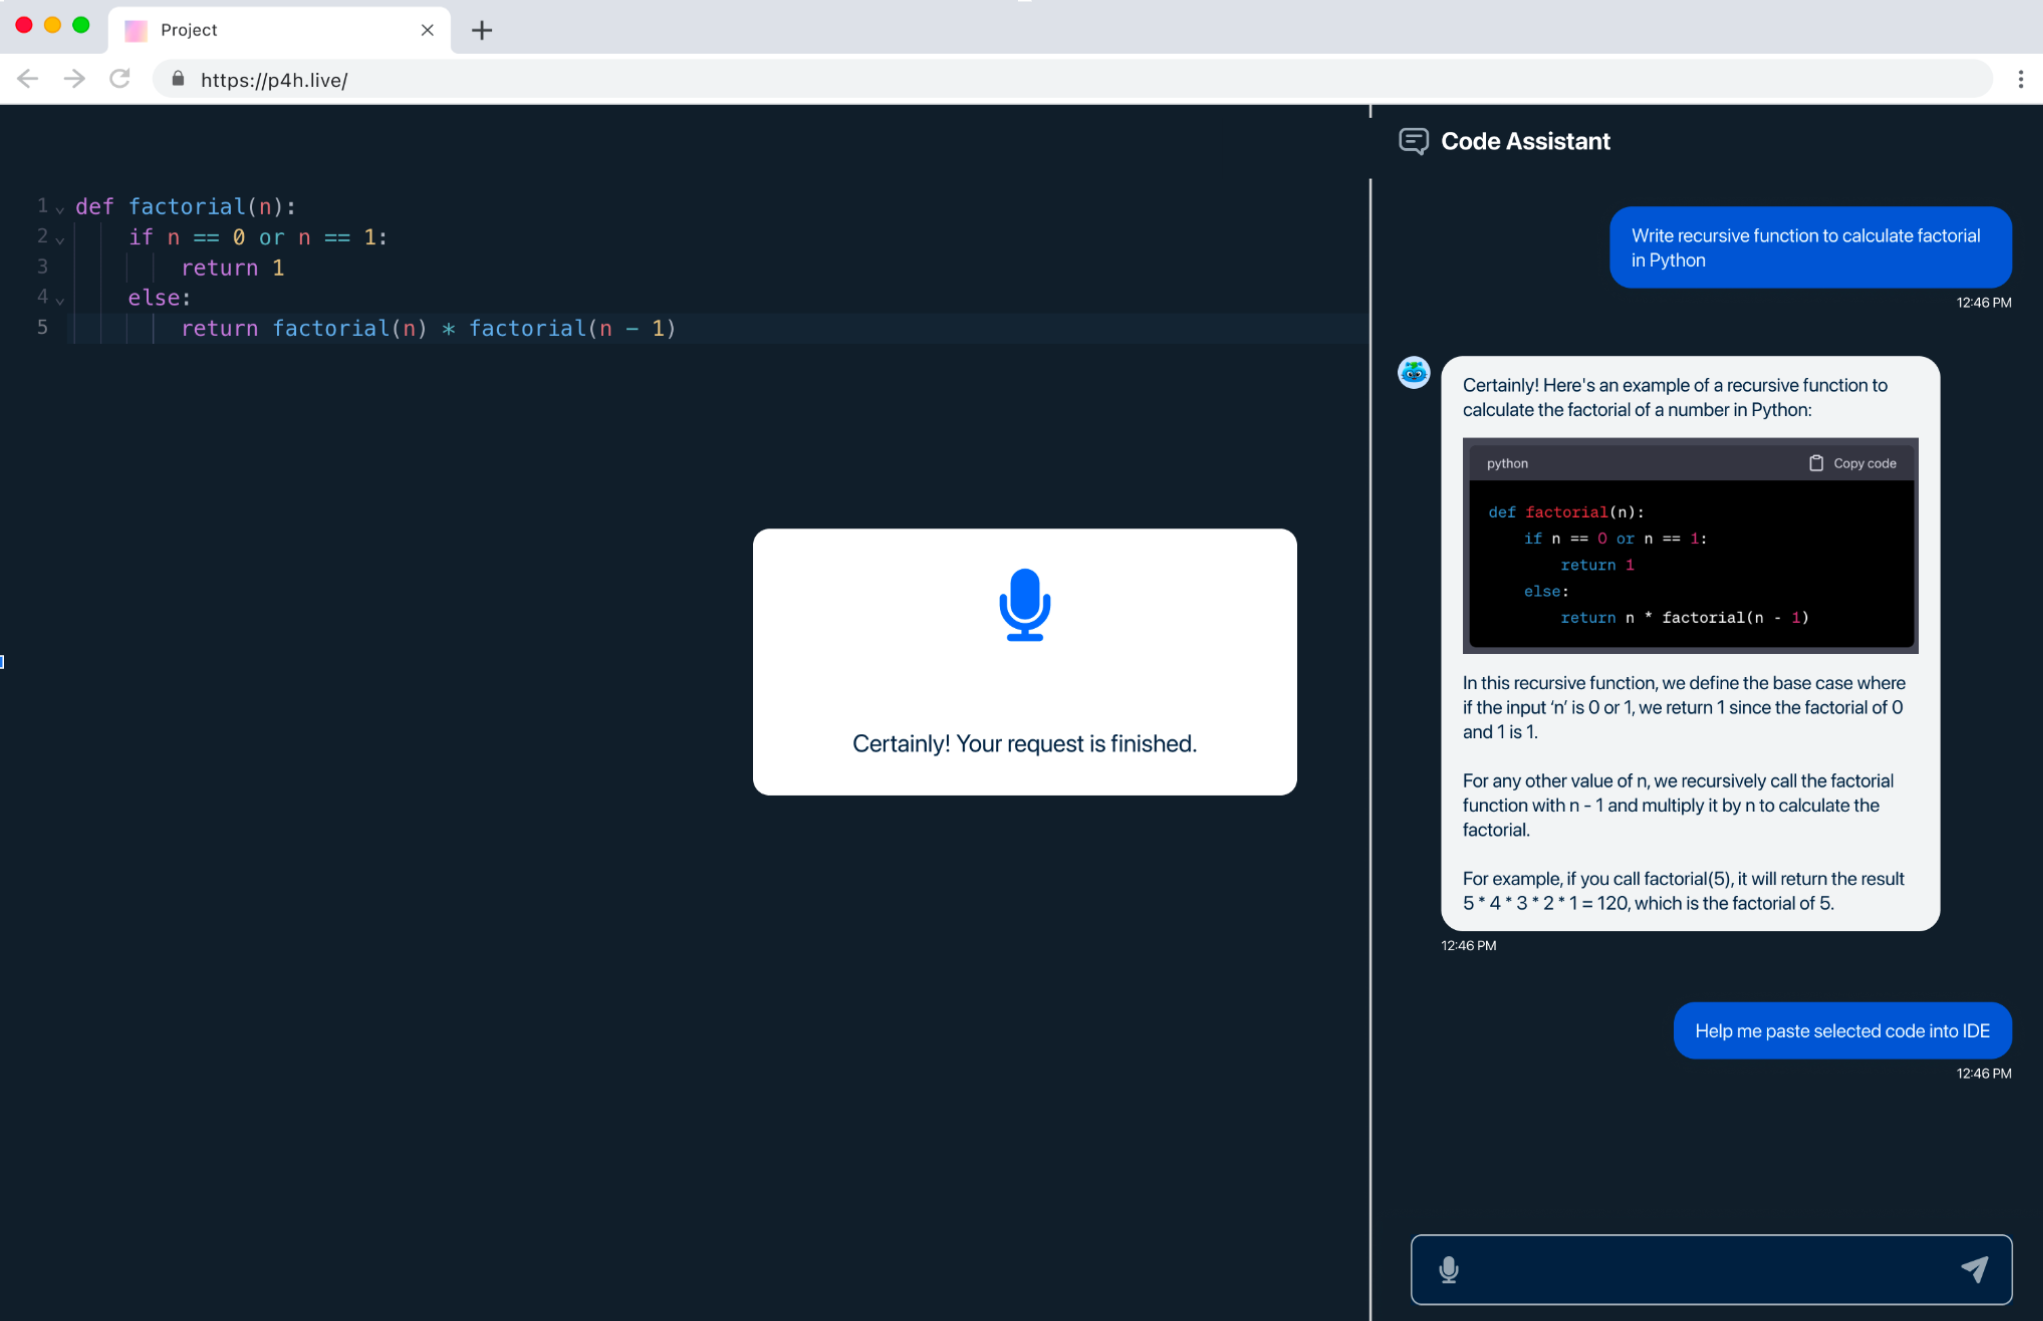
\includegraphics[width=.98\textwidth]{p4h-2}
%\caption{caption 2}
%\label{fig:right}
%\end{figure}
\end{minipage}  
%\vspace{-18pt}
\caption{Voice to Code Generation}
\label{thrust3-one}
\end{figure}

{\bf Voice to Code Generation for Adaptive Learning.} In this use case
scenario (Figure~\ref{thrust3-one}), let's explore how a VIPL
interacts with our proposed environment to create
source code for calculating the factorial of a number. This scenario
showcases the environment's voice interaction and code generation
capabilities.

{\em Initialization}: The visually-impaired programmer initiates the
programming environment by saying, "Hey, Environment, start a new code
project for calculating factorial."

{\em Voice Interaction}: The environment responds with a synthesized voice,
"Sure, please specify the number for which you want to calculate the
factorial." The programmer responds, "Calculate the factorial of 5."

{\em Code Generation}: The programming environment interprets the user's
request and generates the code snippet using advanced voice
recognition and generative AI technologies.  The environment then
communicates, "I've generated the code to calculate the factorial of
5. Here's the code for you:".

{\em Verification}: The generated code is read back to the user through synthesized speech, and the user can confirm its accuracy.
The user says, "Please read back the generated code."

{\em Confirmation}: The environment reads the code aloud, "Def factorial(n): If n equals 0, return 1. Else, return n times factorial(n minus 1). Result equals factorial(5). Print 'The factorial of 5 is:' and the result." The user confirms that the code accurately reflects their intent.

{\em Execution}: The programmer can proceed to execute the code by saying, "Execute the code." The environment executes the code, and the synthesized speech reads the result, "The factorial of 5 is: 120."

{\em Documentation}: The programmer can further enhance the code by documenting it using voice commands. For example, they can say, "Add a comment: This code calculates the factorial of a number."

{\em Integration}: If the programmer has an existing project, they can
integrate this code seamlessly into their project using voice
commands, ensuring a cohesive workflow.

%=========================================================

\begin{figure}[t]
\centering
\begin{minipage}{.48\textwidth}
%\begin{figure}[t]
\centering
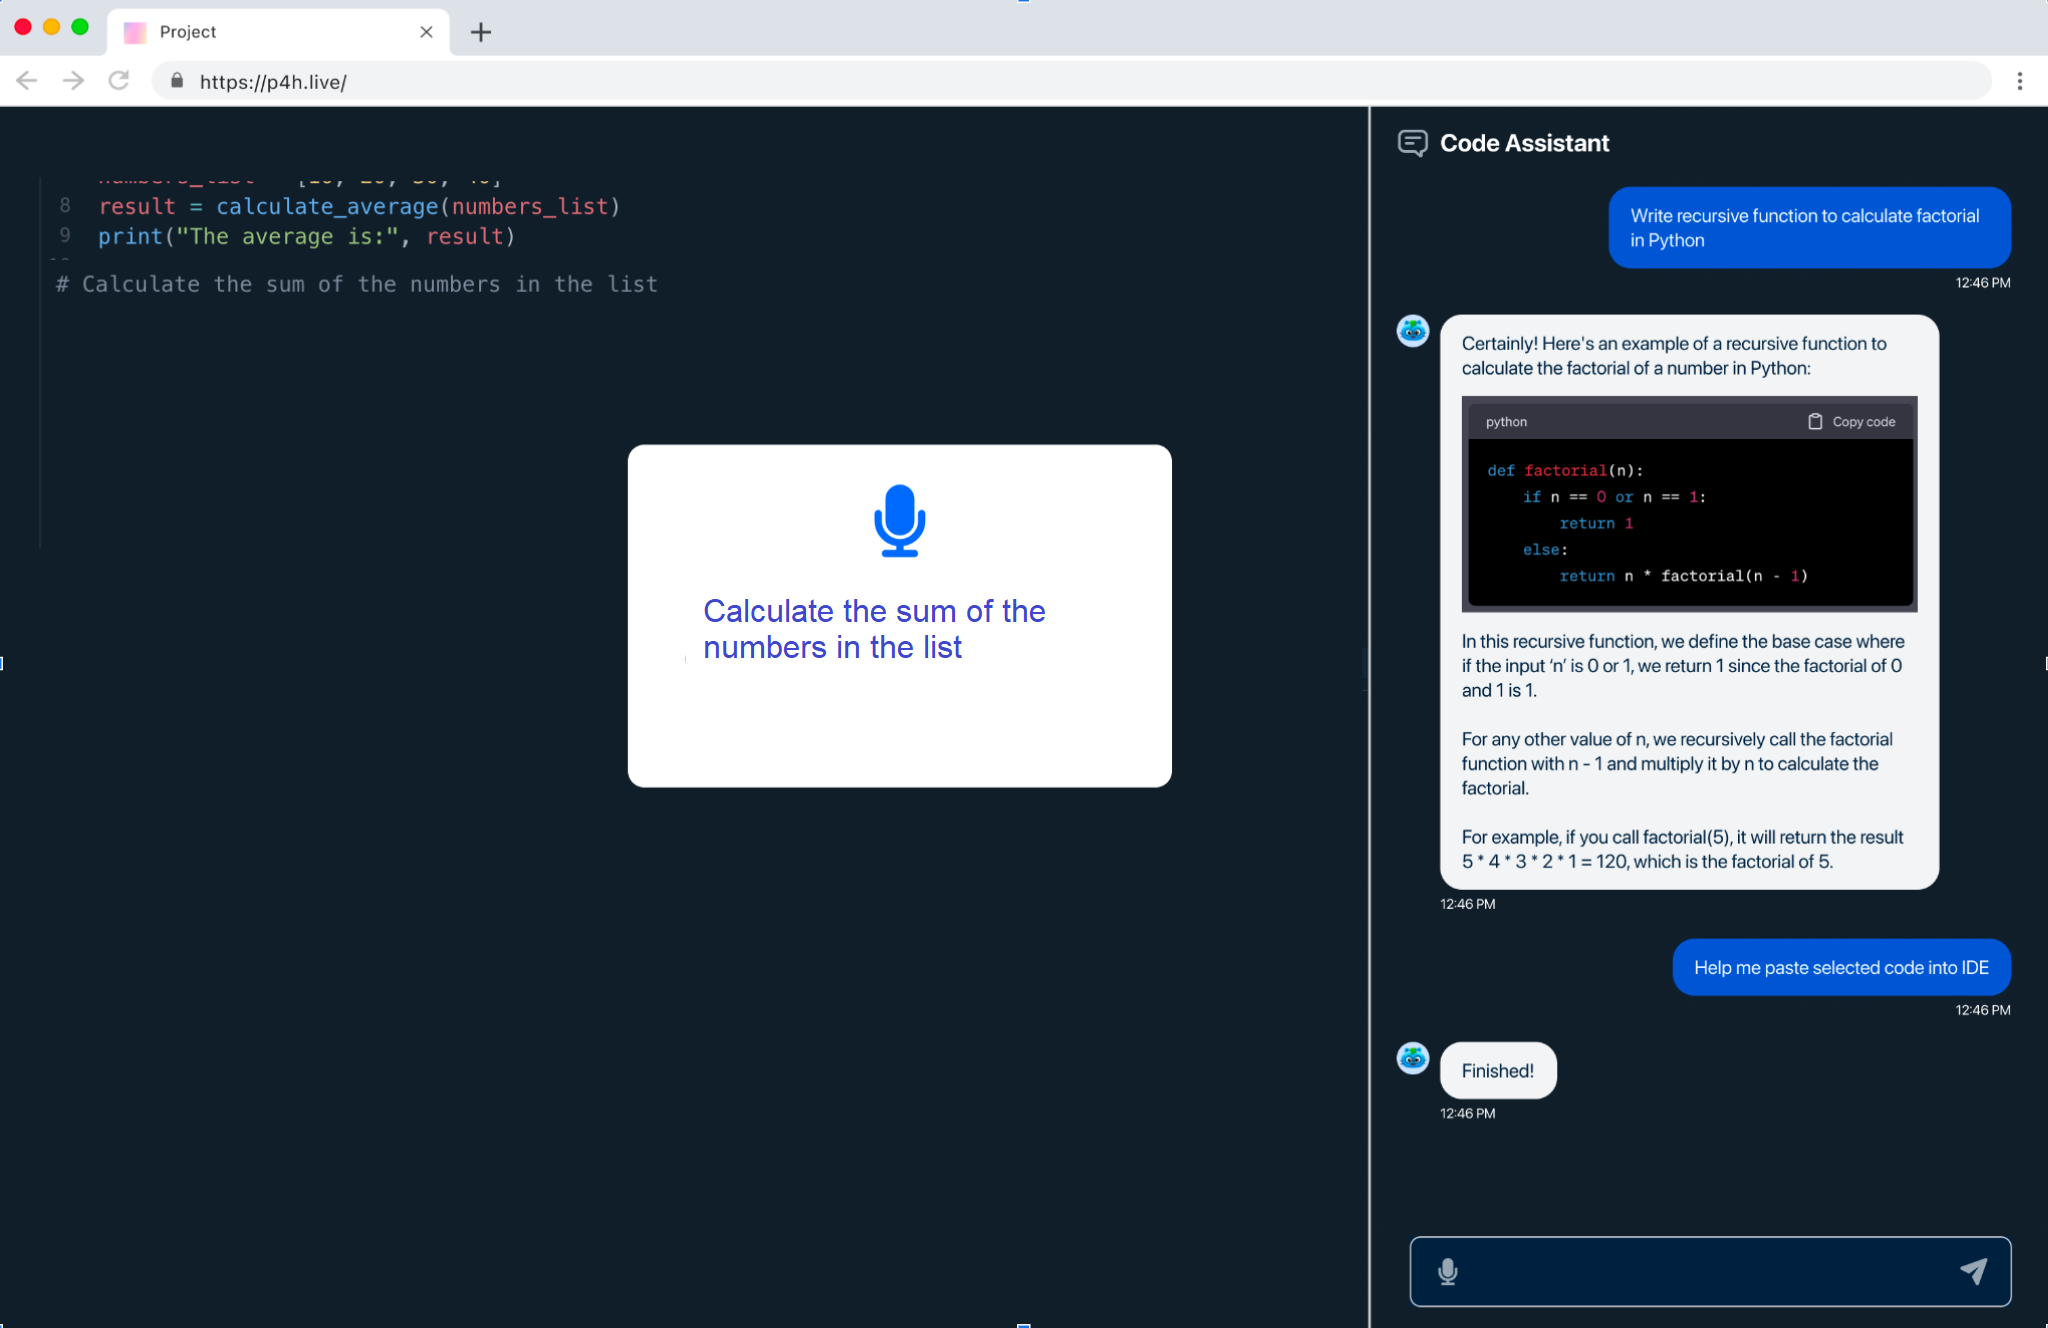
\includegraphics[width=.98\textwidth]{p4h-3}
%\caption{caption 1}
%\label{fig:left}
%\end{figure}
\end{minipage}
\begin{minipage}{.48\textwidth}
%\begin{figure}[t]
\centering
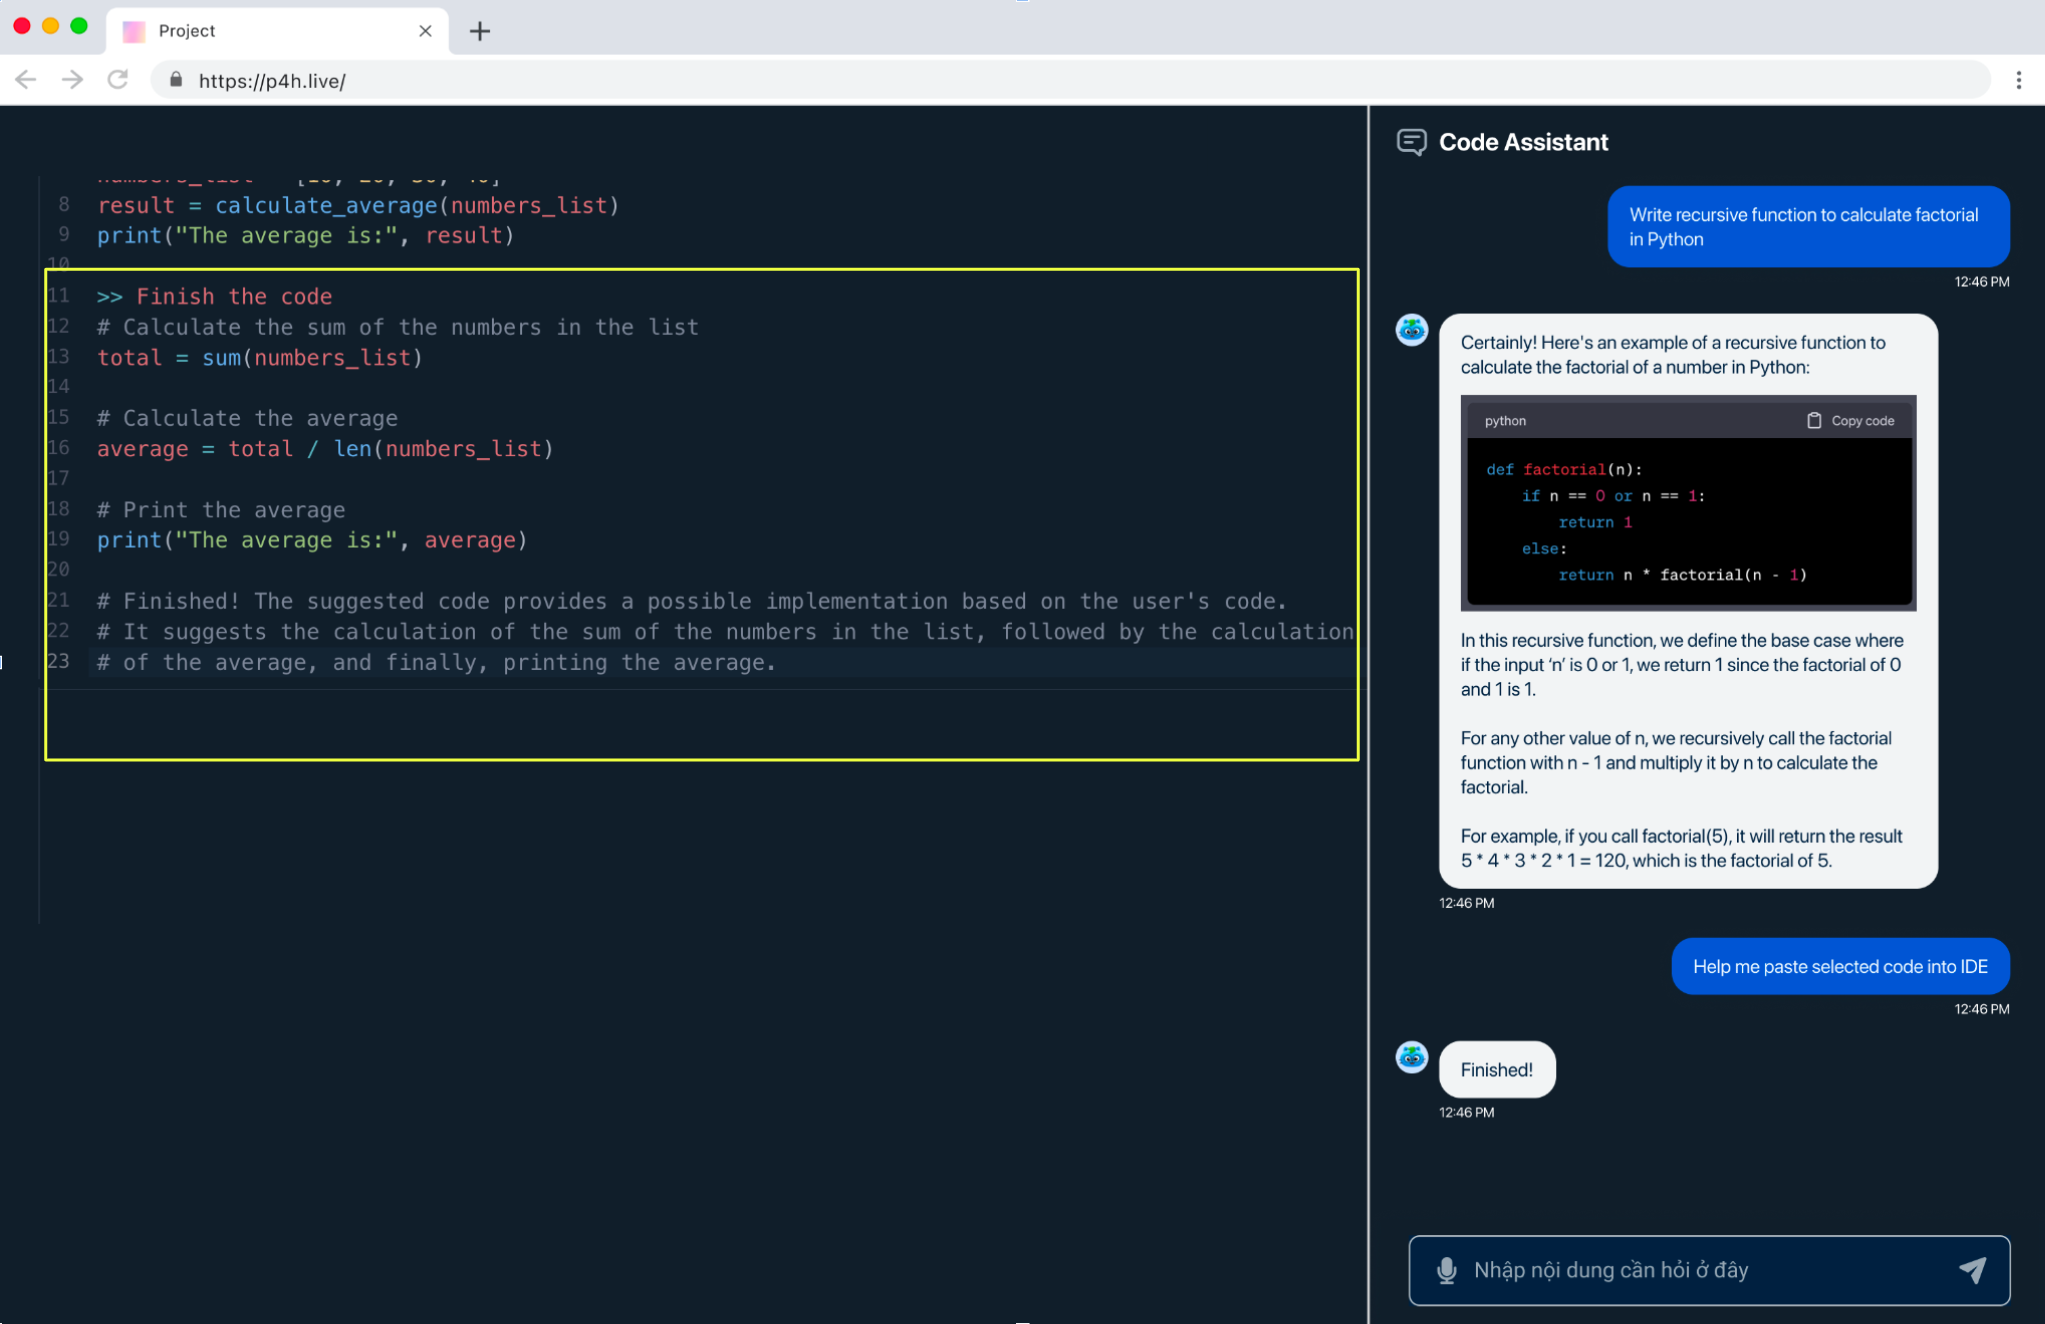
\includegraphics[width=.98\textwidth]{p4h-4}
%\caption{caption 2}
%\label{fig:right}
%\end{figure}
\end{minipage}  
%\vspace{-18pt}
\caption{In-line Voice to Code Generation}
\label{thrust3-two}
\end{figure}

\noindent {\bf Voice for A Programming Task.} Let us consider a scenario in which Sarah
begins her coding session by launching our proposed environment using
voice commands. The platform instantly activates, and she hears a
synthesized voice welcoming her.

{\em Setting Up the First Task: Computing Factorials and Storing in a
  List:} Sarah instructs the environment using natural language voice
commands, "I want to compute the factorial values of numbers from 1 to
100 and store those values in a list."

{\em Voice-to-Code Conversion - First Part:} The environment's
advanced voice recognition technology processes her command and
generates the initial code structure. Sarah continues to articulate
her requirements verbally, "For each number from 1 to 100, calculate
its factorial and add it to the factorial$\_$list."

{\em Real-time Code Generation - First Part}:
The environment translates her voice command into code as shown in Figure~\ref{thrust3-two}.

{\em Verification and Documentation - First Part}: The environment
reads back the generated code to Sarah using synthesized speech. She
listens carefully to ensure that her intent is accurately translated
into code. Satisfied, she decides to generate comprehensive
documentation for this part of her code.

%{\em Integration and Test Cases - First Part:} Impressed with the
%environment's capabilities, Sarah seamlessly integrates her newly
%created code into her existing project, which focuses on mathematical
%computations. She also uses voice commands to create test cases for
%this part of her code.

{\em Requesting the Second Piece of Code: Computing Summation:} Having
successfully completed the first part of her task, Sarah now wants to
compute the summation of the factorial values stored in
factorial$\_$list. She issues a voice command to request the environment
to generate the code for this part of her task.

{\em Voice-to-Code Conversion - Second Part:} The environment
processes her new command and generates the code structure for
computing the summation.
Sarah continues with her voice commands, "Now, calculate the summation
of values in the factorial$\_$list and store it in total$\_$sum."

{\em Real-time Code Generation - Second Part:}
The environment translates her voice command into code.

{\em Verification and Documentation - Second Part:} The environment
reads back the generated code for the summation part. Sarah listens
carefully to ensure accuracy and completeness. Satisfied with the
code, she decides to generate comprehensive documentation for this
part as well.

%{\em Integration and Test Cases - Second Part:} Sarah integrates the
%newly generated code for summation into her existing project, ensuring
%that her project now computes and stores both the factorial values and
%their summation. She also creates test cases for this part of her
%code.

%With the help of this innovative programming environment, Sarah successfully completes her task. She feels empowered, as this environment not only mitigated accessibility barriers but also provided her with a versatile and inclusive toolset for a productive coding journey.
